\documentclass[../main.tex]{subfiles}

% 2.2.1 Wellenverhalten bei Substanzen
Beim zusammenkommen einer Welle mit einer Substanz kann es zu verschiedenen Abschwächungen der Welle kommen. Es spielen Absorption, Streuung, Beugung und Reflexion (Abb. \ref{fig:extinktion_typen}) eine Rolle.

% TODO alternative image (copyright..)
\begin{figure}[ht]
    \centering
    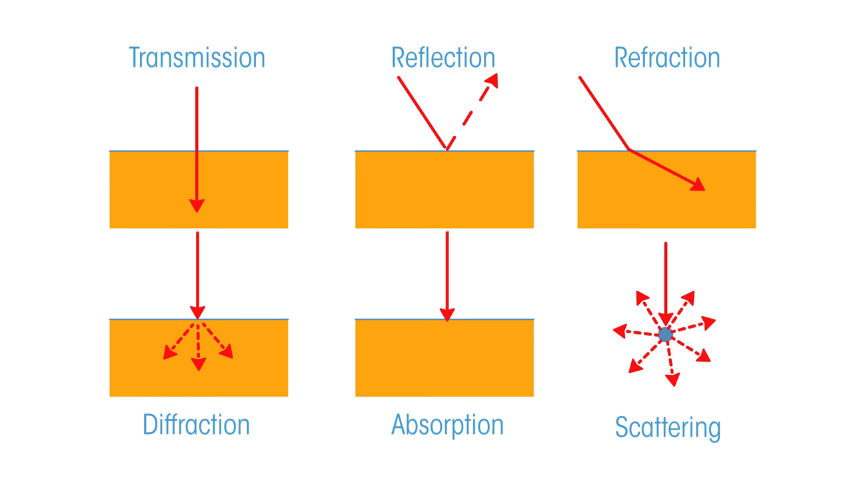
\includegraphics[width=0.65\textwidth]{extinktion_typen.png}
    \caption{Einflussfaktoren auf Extinktion}
    \label{fig:extinktion_typen}
\end{figure}

% 2.2.2 Streuung
\textbf{Streuung} ist die Ablenkung von Wellen in mehrere Richtungen.
% 2.2.3 Beugung
Wenn Strahlungen eine Substanz mit unterschiedlicher Dichte durchqueren, kommt es zu einer Verlangsamung der Ausbreitung, und damit zu einer Richtungsänderung - das ist \textbf{Beugung}.
% 2.2.4 Reflexion
Glatte Oberflächen \textbf{reflektieren} häufig Strahlungen (z.B. Spiegel).

% 2.2.5 Absorption
\textbf{Absorption} beschreibt in der Physik die Aufnahme von Wellen in einer Substanz. Diese ist für die IR-Spektroskopie besonders interresant, da beim Zusammenkommen von Infrarotlicht mit einer Substanz Vibrationsmuster in den Molekülen auftreten, anhand dessen sich der Aufbau der Substanz ableiten lassen kann. Verschiedene funktionelle Gruppen in der Chemie haben nämlich bei verschiedenen Wellenlängen Absorptionseigenschaften. So treten z.B. bei Wasser ($H_2O$) Absorptionen bei \SI{2.734}{\micro\metre}, \SI{6.269}{\micro\metre} und \SI{2.662}{\micro\metre} auf. Die Vibrationsmuster sind jeweilig symmetrisches Dehnen der $OH$-Bindungen (Abb. \ref{fig:oh_symmetric_stretching}), $H-O-H$-Beugung (Abb. \ref{fig:hoh_bending}) und $OH$-asymetrisches Dehnen (Abb. \ref{fig:oh_asymmetric_stretching}).

\begin{figure}
    \centering
    \begin{subfigure}[b]{0.3\textwidth}
        \chemfig{
            O(-[:135,0.8]H)(-[:45,0.8]H)
        }
        \hspace{0.1cm}
        \chemfig{
            O(-[:135,1.2]H)(-[:45,1.2]H)
        }
        \caption{OH Symmetrisches Dehnen}
        \label{fig:oh_symmetric_stretching}
    \end{subfigure}
    \begin{subfigure}[b]{0.3\textwidth}
        \chemfig{
            O(-[:135]H)(-[:45]H)
        }
        \hspace{0.1cm}
        \chemfig{
            O(-[:160]H)(-[:20]H)
        }
        \caption{HOH Beugung}
        \label{fig:hoh_bending}
    \end{subfigure}
    \begin{subfigure}[b]{0.3\textwidth}
        \chemfig{
            O(-[:135,1.2]H)(-[:45,0.8]H)
        }
        \hspace{0.1cm}
        \chemfig{
            O(-[:135,0.8]H)(-[:45,1.2]H)
        }
        \caption{OH Asymmetrisches Dehnen}
        \label{fig:oh_asymmetric_stretching}
    \end{subfigure}
    \caption{Vibrationsmuster}
\end{figure}

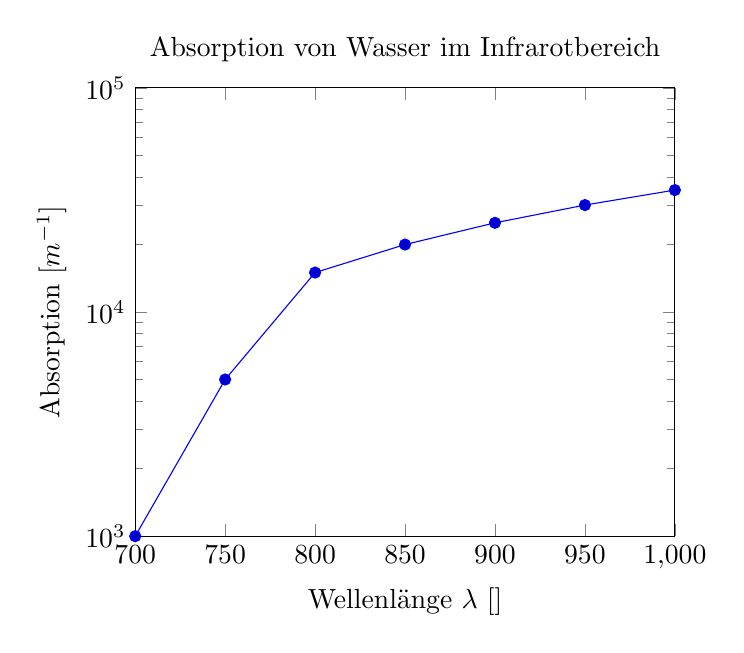
\begin{tikzpicture}
    \centering
    \begin{axis}[
        title={Absorption von Wasser im Infrarotbereich},
        xlabel={Wellenlänge $\lambda$ [\SI{}{\micro\metre}]},
        ylabel={Absorption [$m^{-1}$]},
        xmin=700, xmax=1000,
        ymin=1000, ymax=100000, ymode=log,
    ]

    \addplot table { % TODO real values
            700 1000
            750 5000
            800 15000
            850 20000
            900 25000
            950 30000
            1000 35000
        };
    \end{axis}
\end{tikzpicture}